
\bigbreak
\bigbreak
\bigbreak
\bigbreak
\section{General Architecture}\label{sec:general-arcitecture}
The general architecture of this implementation is as follows:
\begin{enumerate}
    \item \textbf{data extraction}: The position metrics, timestamp and coordinates, of the user's mouse cursor are collected from the user's computer and sent to the server for analysis. The \textit{Dataset} section~\ref{sec:dataset} outlines this stage.
    \item \textbf{features generation}: From the inputted raw data recorded and sent from the user's machine, features that characterize the raw data, and the user's session pertaining to it, are generated. The \textit{Features Engineering} section~\ref{sec:features-engineering} outlines this stage.
    \item \textbf{clustering}: Sessions are clustered based on the generated features. The \textit{Clustering} section~\ref{sec:clustering} outlines this stage.
    \item \textbf{classification}: Clusters of sessions are used to determine bottness of users at client IP addresses. The \textit{Classification} section~\ref{sec:classification} outlines this stage, a stage anticipated for future work.
\end{enumerate}
\begin{figure}[!h]
    \centering
    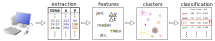
\includegraphics[width=1\columnwidth]{figures/general_architecture}
    \caption{Architecture of this bot detection scheme}
    \label{fig:general-architecture}
\end{figure}

The \textit{Implementation} chapter~\ref{ch:implementation} described how this architecture is built.
